% This is a template for Ph.D. dissertations in the UCI format.
% 
% All fonts, including those for sub- and superscripts, must be 10
% points or larger.  Recommended sizes are 14-point for chapter
% headings, 12-point for the main body of text and figure/table
% titles, and 10-point for footnotes, sub- and super-scripts, and text
% in figures and tables.
%
% Notes: Add short title to figures, sections, via square brackets,
% e.g. \section[short]{long}.
%
\documentclass[12pt,fleqn]{ucithesis}

% A few common packages
\usepackage{amsmath}
\usepackage{amsthm}
\usepackage{array}
\usepackage{graphicx}
\usepackage{natbib}
\usepackage{relsize}

% Some other useful packages
\usepackage{caption}
\usepackage{subcaption}  % \begin{subfigure}...\end{subfigure} within figure
\usepackage{subfloat} 
\usepackage{multirow}
\usepackage{tabularx}

% plainpages=false fixes the "duplicate ignored" error with page counters
% Set pdfborder to 0 0 0 to disable colored borders around PDF hyperlinks
\usepackage[plainpages=false,pdfborder={0 0 0}]{hyperref}

% Uncomment the following two lines to use the algorithm package,
% which provides an algorithm environment similar to figure and table
% ("\begin{algorithm}...\end{algorithm}"). A list of algorithms will
% automatically be added in the preliminary pages. Note that you
% probably want a package for the actual code to go with this (e.g.,
% algorithmic).
%\usepackage{algorithm}
%\renewcommand{\listalgorithmname}{\protect\centering\protect\Large LIST OF ALGORITHMS}

% Uncomment the following line to enable Unicode support. This will allow you
% to enter non-ASCII characters (such as accented characters) directly without
% having to use LaTeX's awkward escape syntax (e.g., \'{e})
% NOTE: You may have to install the ucs.sty package for this to work. See:
% http://www.unruh.de/DniQ/latex/unicode/
%\usepackage[utf8x]{inputenc}

% Uncomment the following to avoid "widowing", where page breaks cause
% single lines of paragraphs to float onto the next page (this is not
% a UCI requirement but more of an aesthetic choice).
%\widowpenalty=10000
%\clubpenalty=10000

% Modify or extend these at will.
\newtheorem{theorem}{\textsc{Theorem}}[chapter]
\newtheorem{definition}{\textsc{Definition}}[chapter]
\newtheorem{example}{\textsc{Example}}[chapter]
\newcommand{\mychapter}[2]{
    \setcounter{chapter}{#1}
    \setcounter{section}{0}
    \chapter*{#2}
    \addcontentsline{toc}{chapter}{#2}
}

% Macros for title, author, abstract, etc.
\thesistitle{Investigating Macroscopic Physiology of the Human Brain to Study Sleep Homeostasis and its Effect on Disease and Cognition}

%"Dissertation" for PhD, "Thesis" for master's
\documenttitle{Advancement}

\degreename{Doctor of Philosophy}

% Use the wording given in the official list of degrees awarded by UCI:
% http://www.rgs.uci.edu/grad/academic/degrees_offered.htm
\degreefield{Mathematical and Computational Systems Biology}

% Your name as it appears on official UCI records.
\authorname{Logan Davendra Harriger}

% Use the full name of each committee member.
\committeechair{Michael A. Yassa}
\othercommitteemembers
{
  Jack J. Lin\\
  Bruce J. Tromberg\\
  Norbert J. Fortin\\
  Bryce A. Mander
}

\degreeyear{2018}

\copyrightdeclaration
{
  {\copyright} {\Degreeyear} \Authorname
}

% If you have previously published parts of your manuscript, you must list the
% copyright holders; see Section 3.2 of the UCI Thesis and Dissertation Manual.
% Otherwise, this section may be omitted.
% \prepublishedcopyrightdeclaration
% {
% 	Chapter 4 {\copyright} 2003 Springer-Verlag \\
% 	Portion of Chapter 5 {\copyright} 1999 John Wiley \& Sons, Inc. \\
% 	All other materials {\copyright} {\Degreeyear} \Authorname
% }

% The dedication page is optional
% (comment out to exclude).
\dedications
{
  (Optional dedication page)
  
  To ...
}

\acknowledgments
{
  I would like to thank everyone who has supported me in the challenging, twisted, and uncertain journey that eventually grants a PhD.
  
  Advisor and mentor, Mike Yassa.
  Mentor, Jack Lin.
  Other members of advancement committee. Especially Bryce Mander for introducing me to the field of sleep science, scoring sleep records, and many insightful discussions. 
  
  Yassa Lab. Rebbecca Stevenson, Freddie Marquez, and Steve Granger
  Director of CNLM ambassadors, Manuella Yassa.
  
  Program for Mathematical, Computational, and Systems Biology. Especially, my incoming cohort.
  
  Center for Complex Biological Systems
  
  You must acknowledge grants and other funding assistance. 

}

% Some custom commands for your list of publications and software.
\newcommand{\mypubentry}[3]{
  \begin{tabular*}{1\textwidth}{@{\extracolsep{\fill}}p{4.5in}r}
    \textbf{#1} & \textbf{#2} \\ 
    \multicolumn{2}{@{\extracolsep{\fill}}p{.95\textwidth}}{#3}\vspace{6pt} \\
  \end{tabular*}
}
\newcommand{\mysoftentry}[3]{
  \begin{tabular*}{1\textwidth}{@{\extracolsep{\fill}}lr}
    \textbf{#1} & \url{#2} \\
    \multicolumn{2}{@{\extracolsep{\fill}}p{.95\textwidth}}
    {\emph{#3}}\vspace{-6pt} \\
  \end{tabular*}
}

% Include, at minimum, a listing of your degrees and educational
% achievements with dates and the school where the degrees were
% earned. This should include the degree currently being
% attained. Other than that it's mostly up to you what to include here
% and how to format it, below is just an example.
%
% CV is required for PhD theses, but not Master's
% comment out to exclude
% \curriculumvitae
% {

% \textbf{EDUCATION}
  
%   \begin{tabular*}{1\textwidth}{@{\extracolsep{\fill}}lr}
%     \textbf{Doctor of Philosophy in Computer Science} & \textbf{2012} \\
%     \vspace{6pt}
%     University name & \emph{City, State} \\
%     \textbf{Bachelor of Science in Computational Sciences} & \textbf{2007} \\
%     \vspace{6pt}
%     Another university name & \emph{City, State} \\
%   \end{tabular*}

% \vspace{12pt}
% \textbf{RESEARCH EXPERIENCE}

%   \begin{tabular*}{1\textwidth}{@{\extracolsep{\fill}}lr}
%     \textbf{Graduate Research Assistant} & \textbf{2007--2012} \\
%     \vspace{6pt}
%     University of California, Irvine & \emph{Irvine, California} \\
%   \end{tabular*}

% \vspace{12pt}
% \textbf{TEACHING EXPERIENCE}

%   \begin{tabular*}{1\textwidth}{@{\extracolsep{\fill}}lr}
%     \textbf{Teaching Assistant} & \textbf{2009--2010} \\
%     \vspace{6pt}
%     University name & \emph{City, State} \\
%   \end{tabular*}

% \pagebreak

% \textbf{REFEREED JOURNAL PUBLICATIONS}

%   \mypubentry{Ground-breaking article}{2012}{Journal name}

% \vspace{12pt}
% \textbf{REFEREED CONFERENCE PUBLICATIONS}

%   \mypubentry{Awesome paper}{Jun 2011}{Conference name}
%   \mypubentry{Another awesome paper}{Aug 2012}{Conference name}

% \vspace{12pt}
% \textbf{SOFTWARE}

%   \mysoftentry{Magical tool}{http://your.url.here/}
%   {C++ algorithm that solves TSP in polynomial time.}

% }

% The abstract should not be over 350 words, although that's
% supposedly somewhat of a soft constraint.
\thesisabstract
{
  The abstract of your contribution goes here.
}


%%% Local Variables: ***
%%% mode: latex ***
%%% TeX-master: "thesis.tex" ***
%%% End: ***


% Add PDF document info fields
\hypersetup{
	pdftitle={\Thesistitle},
	pdfauthor={\Authorname},
	pdfsubject={\Degreefield},
}

% Uncomment the following to have numbered subsubsections (by default
% numbering goes only to subsections).
%\setcounter{secnumdepth}{4}


% Set this to only select a subset of the includes directives below.
% Very handy to speed up compilation if you're working on a certain
% part of your thesis. It conserves page numbers, references, etc.
% even for non-included files.
%\includeonly{chapter1}

%\bibpunct{}{}{,}{s}{,}{,}
\bibpunct{(}{)}{;}{a}{,}{,}
%\citestyle{nature}


\begin{document}

% Preliminary pages are always loaded (TOC, CV, etc.)
\preliminarypages

% Include the different components of your thesis, in separate files.
% Using \include allows you to set \includeonly above.
\mychapter{1}{Specific Aims}

% Aim 1: Identify changes in brain network activity as a function of sleep state.
% Aim 2: Examine sleep processes supporting biographical memories
% Aim 3: Develop MRI method to quantify brain-wide CSF flow dynamics as a function of brain state

The consequences of sleep deprivation are a growing list including loss of sex drive, elevated blood pressure, weakened immunity, cognitive impairment, and increased risk for a wide range of diseases. So while unconsciousness is the most obvious feature of sleep, it is just a side-effect of this profound state change which facilitates critical homeostatic processes throughout the body - especially in the brain. Around sleep onset, movement and sensory stimulation are reduced along with the demand for oxygen in tissues serving these functions, thus permitting respiration to slow and the heart relax. As the brain falls deeper into sleep, the concentration of neuromodulatory transmitters, like norepinephrine and serotonin, decrease, and neuronal activity alternates between active and inactive firing states modulated by $\sim$1 Hz waveforms called slow waves (SW). In parallel, astrocytes reduce their rate of lactate production, seek out synapses to phagocytose, alter ionic composition and permit greater flow of extracellular cerebrospinal fluid (CSF) through the brain. Importantly, these sleep processes and others have strong connections to cognition, aging, and disease, but some of these findings are inadequately studied in humans mostly limited by suitable methods that also meet the paramount ethical considerations for studying human subjects.
% Traveling waves evident in VSD, replay evident from dense micro-electrodes, and glymphatic activity.

One path forward is to combine existing techniques with novel analyses. I propose using combinations of structural, functional, and flow magnetic resonance imaging (MRI) as well as electroencephalography (EEG) to examine how fluid and electrical dynamics are organized by the brain to support sleep homeostasis, and determine how these dynamics are altered by learning, age, and dementia. While the majority of these techniques can be readily utilized with available resources, I am currently piloting a phase-contrast MRI (pcMRI) sequence to extend its application to the measurement of low-velocity extracellular CSF flow; however, the feasibility of this application is supported by the routine use of pcMRI to measure higher velocity flow of blood and CSF in larger structures as well as our initial pilot data. By utilizing several ongoing or imminent collaborations, I will have access to unique subject populations including: (1) epilepsy patients implanted with intracranial EEG (iEEG), (2) patients with varying degrees of dementia who will participate in MRI and potentially scalp EEG studies, (3) patients with sleep dysfunction who will participate in EEG and potentially MRI studies, and (4) healthy controls who would participate in MRI and EEG studies. There already exists a large repository of iEEG recordings in subjects from (1) during sleep and wake, which is currently being utilized to address Aim 1, and given subject throughput of our existing collaborations, I should be able to collect sufficient data for the remaining aims in about a year.

% Collecting adequate data should be possible within 1-2 years by leveraging 
%, integrating information from multiple modalities to contextualize data in a more natural and comprehensive space
\textbf{\textit{Aim 1 will identify basic changes in brain network activity as a function of sleep state.}} Intracranial electrodes will be localized to the brain using CT and MRI, and spontaneous recordings will be analyzed to assess how spatiotemporal dynamics of SW activity differ between sleep and wake. This will also be applied to the spindle band to further evaluate how SW and spindle networks couple in space and time. 

\textbf{\textit{Aim 2 is to examine how sleep processes support biographical memories.}} An audio-visual name-face association task will be administered to subjects before and after sleep. Memory performance will be correlated with various metrics for sleep quality and depth. Additionally, I will identify task relevant brain network dynamics in a variety of contexts including stimulus presentation, partial presentation (name or face), imagination, and the presentation of name audio clips during sleep. Finally, spontaneous sleep recordings will be analyzed for evidence of reactivation of these brain networks.      

\textbf{\textit{Aim 3 will extend existing MRI methods to quantify brain-wide CSF flow dynamics as a function of brain state.}} Flow of CSF through the brain parenchyma is regulated by the glymphatic system, which is formed by astrocytes. This glymphatic activity substantially increases during SWS promoting the clearance of toxins like amyloid-$\beta$, and therefore may be a mechanistic factor in Alzheimer's disease (AD).  To provide a translational link to this line of research, I propose using phase-contrast MRI to quantify changes in CSF flow between wake and sleep; additionally, I evaluate whether this flow is disrupted in patients with AD.  

%- which is routinely used to measure blood and CSF flow in large structures with velocities $>$10cm/s to show evidence of glymphatic activity in humans. 

% During sleep, animals lose awareness of the environment as well as their will to affect it, but this cost of losing of touch is accompanied by a provisional guarantee on the stability for the body: by drastically limiting its interaction with the environment, the body can refocus its energy on other needs, such as growth, repair, and cleanup. The value of this process might be appreciated in terms of the consequences of sleep deprivation - a long list including, loss of sex drive, weakened immunity, increased blood pressure, and cognitive impairment, to name as few. Around sleep onset, movement and sensory stimulation decrease, along with the demand for oxygen by the tissues serving these functions, thus permitting respiration to slow and the heart relax. As the brain falls deeper into sleep, neuronal activity is increasingly modulated at low-frequency cycles around 1 Hz called slow waves (SW) oscillating between inactive and active firing states. In parallel, glia, especially astrocytes undergo a major shift in activity; for example, altering ionic composition and permitting greater flow of interstitial fluid, reducing their rate of lactate production, increasing phagocytosis of damaged neural components.
%Importantly, during sleep as well as wake, neurons do not operate in isolation, but are supported by the entire body, and most intimately by its direct relatives the glia. Yet despite this critical dependence, studies of the human brain have a tendency to fixate on neural factors.
%While this dependence may be negligible on short-time scales 



%%


% Many has been discovered about sleep processes, but 
% integration, extend to humans, translational, 

%While cells do have a functional specialization, they are not isolated.
%However, periodically, sleep will shift into another state, in which neural activity more closely resembles wake. 
%there is a slowing in neural activity: among other changes, 
%discount the activity of non-neuronal tissue.
%[and becomes less interdependent]
%the body generally slows, for instance, 

%These slow waves are closely related to unconsciousness, but mental state is only one effect of sleep. 
%Due to special ethical considerations for studying human subject? Perhaps it is conceptually simpler? 
%The development of the brain is a story of neurons and glia eventually emerging together as daughters of the gastrula's neural crest cells. These cells organize themselves into a complex pattern harmonizing with the parallel development of the vascular system and overcoming space constraints of the skull by folding as it continues to expand. Of course, this development does not stop after birth, but continues, albeit in a different way, as the organism adapts an environment and body in constant change.

%Like the rest of nature, the life of an organism consists of persistent cycles interweaving with one another to support the whole.
%Sleep is a profound change in our state of consciousness, but also the functioning of our body.

%fMRI: Neural representation of 2D objects VS hemodynamic response to visual stimulation 
%to adopt a neuro-centric perspective, in which the non-nervous tissues 
% are considered in relative isolation, only interacting with each other
%place little emphasis on studying interaction of the nervous system. 

%Aim 2: Evaluate physiological responses supporting multi-sensory association task memory processes and during sleep.}
%reactivation in audio-visual paired-association task.}
%Develop phase-contrast magnetic resonance imaging methods to quantify glymphatic activity in human brain.}
%Effective network connectivity indicated by wave propagation patterns.

%%% Local Variables: ***
%%% mode: latex ***
%%% TeX-master: "thesis.tex" ***
%%% End: ***

\mychapter{2}{Introduction}
%
% Problems and objectives of your research should be clearly stated and placed in the context of a broader field. An extensive bibliography should be included. This section should lead the reader to each question or hypothesis that you’re testing in each aim. Significance of the project should be also included here.
%
During sleep, animals lose awareness of the environment as well as their will to affect it, but this cost of losing of touch is accompanied by a provisional guarantee on the stability of the body: by drastically limiting its interaction with the environment, the body can refocus its energy on other needs, such as growth, cleanup, and repair. The value of this process might be appreciated in terms of the consequences of sleep deprivation - a long list including, loss of sex drive, weakened immunity, increased blood pressure, memory impairment, and increased risk for many diseases like Alzheimer's dementia (AD). So while unconsciousness is the most obvious feature of sleep, it is just a side-effect of this profound state change which facilitates critical homeostatic processes throughout the body - especially in the brain. Around sleep onset, movement, sensation, and cognition are reduced along with the metabolic demand in tissues serving these functions, thus permitting respiration to slow and the heart relax. As the brain falls deeper into sleep, the concentration of neuromodulatory transmitters, like norepinephrine and serotonin, decrease, and neuronal activity increasingly alternates between active and inactive firing states modulated by $\sim$1 Hz waveforms called slow waves (SW). In parallel, glia, especially astrocytes, undergo a major shift in activity; for example, altering ionic composition and permitting greater flow of interstitial fluid, reducing their rate of lactate production, and increasing phagocytosis of fatigued neural components. Determining how the function and dysfunction of these processes promote and reduce brain health will improve our basic understanding of sleep and may introduce new therapeutic targets. With my dissertation, I hope to contribute to the science of human slow wave sleep by identifying patterns of macroscopic electrophysiology that support memory consolidation and by imaging glymphatic activity to evaluate its role in aging and dementia. Below, I begin with a broad survey of the literature relevant to slow wave sleep and its relationship to memory, aging, and dementia.
%!!!%

%%%%%%%%%%%%%%%%%%%%%%%%%%%%%%%%%%%%%%%%%%%%%%%%%%%%%%%%%%%%%%%%%%%%%%%%%%%%%%%%%%%%
%%%%%%%%%%%%%%%%%%%%%%%%%%%%%%%%%%%%%%%%%%%%%%%%%%%%%%%%%%%%%%%%%%%%%%%%%%%%%%%%%%%%
\section*{Sleep staging}
%%%%%%%%%%%%%%%%%%%%%%%%%%%%%%%%%%%%%%%%%%%%%%%%%%%%%%%%%%%%%%%%%%%%%%%%%%%%%%%%%%%%
%%%%%%%%%%%%%%%%%%%%%%%%%%%%%%%%%%%%%%%%%%%%%%%%%%%%%%%%%%%%%%%%%%%%%%%%%%%%%%%%%%%%
Sleep stages were defined by Allan Rechtschaffen and Anthony Kales in 1968 based on a method of evaluating polysomnography (PSG) comprised of three types of recordings: (1) electroencephalogram (EEG) derived from at least two electrodes placed near the center of the scalp to measure brain activity, (2) electrooculogram (EOG) ideally placed above and below the eyes to measure eye movements, (3) electromusculogram (EMG) ideally placed on and beneath the chin to measure general muscle tone \citep{Kales1968}. These three signals are then visually evaluated to stage sleep in 30 second epochs roughly according to the descriptions below:
\begin{enumerate}
\item[] Stage 1: Non-REM stage 1, abbreviated as NREM1, is a transitory stage of sleep onset and might be characterized as a drowsy restfulness. During this period eye movement slows and muscle tone begins to decrease. Also during this stage, the 8-12Hz alpha rhythm usually present when an awake subject closes their eyes begins to disappear; however, brief bursts of a slightly higher frequency around 12-14 Hz, but with lower voltage, called spindles, may be evident.
\item[] Stages 2-4: NREM2-4 are increasing depths of sleep. Starting with NREM2, the most prominent feature of sleep, the slow wave (SW), begins to emerge and persist through NREM4, which is why these three stages are collectively referred to as slow wave sleep (SWS). The incidence of SWs per 30 sec epoch defines the depth of sleep with thresholds of $<20\%$, $20-50\%$, $>50\%$ defining NREM2-4, respectively. Additionally, during NREM2 and 3, spindles (12-14 Hz at least .5 sec in duration) may be present.
\item[] Stage 5: Rapid eye movement, or REM sleep, has also been called paradoxical sleep because it significantly deviates from the EEG patterns observed during NREM, and rather appears with low-voltage mixed-frequency signals very similar to a waking EEG. However, this paradoxical activity can be distinguished with the rest of the PSG since muscle tone remains low, but eye movement becomes rapid.
%\item[] Stage 6: Wake, finally, is distinguished with a high muscle tone, moderate eye movement, and a low-voltage mixed frequency signal, possibly including alpha oscillations.
\end{enumerate}
In addition to these five sleep stages, are criteria for marking epochs during wake, movements, or obscured by too many artifacts to properly score.

%%%%%%%%%%%%%%%%%%%%%%%%%%%%%%%%%%%%%%%%%%%%%%%%%%%%%%%%%%%%%%%%%%%%%%%%%%%%%%%%%%
%%%%%%%%%%%%%%%%%%%%%%%%%%%%%%%%%%%%%%%%%%%%%%%%%%%%%%%%%%%%%%%%%%%%%%%%%%%%%%%%%%
\section*{The slow wave}
%%%%%%%%%%%%%%%%%%%%%%%%%%%%%%%%%%%%%%%%%%%%%%%%%%%%%%%%%%%%%%%%%%%%%%%%%%%%%%%%%%
%%%%%%%%%%%%%%%%%%%%%%%%%%%%%%%%%%%%%%%%%%%%%%%%%%%%%%%%%%%%%%%%%%%%%%%%%%%%%%%%%%
The namesake for slow wave sleep is naturally its most distinctive feature. Although this waveform is well-studied, there is still uncertainty about how to define it, which brain regions generate it, and the mechanisms that give rise to it. 

%%%%%%%%%%%%%%%%%%%%%%%%%%%%%%%%%%%%%%%%%%%%%%%%%%%%%%%%%%%%%%%%%%%%%%%%%%%%%%%%%%%%
\subsection{Slow waves and oscillations}
%%%%%%%%%%%%%%%%%%%%%%%%%%%%%%%%%%%%%%%%%%%%%%%%%%%%%%%%%%%%%%%%%%%%%%%%%%%%%%%%%%%%
This waveform was initially defined by R$\&$K to be between .5-2 Hz, but it also common to define the band as $<1$, $.1-1$, or $1-4$ Hz, and further complicating the terminology are the additional distinctions of delta waves, infraslow waves, and slow oscillations \citep{Amzica1995a, Vyazovskiy2013,Crunelli2010, Crunelli2018}. The SW was first observed in scalp EEG and interpreted as globally synchronized brain activity, but in 1993, a series of papers by Steriade and colleagues demonstrated that neuronal membrane potentials were modulated at a low frequencies with depolarizing/hyperpolarizing phases, which they defined as $<1$ Hz and called a slow oscillation (SO), and coincident with low frequency waveforms in the field potentials \citep{Steriade1993,Steriade1993a,Steriade1993b}. It is worth noting that the frequency range for the SO defined by Steriade is enormous, covering any periodic activity lasting longer than 1 sec, but while dubious, is still frequently used. This unfortunate because recent research efforts have identified activity $<.1$ Hz, to be distinct from the SO \citep{Mitra2014, Schwalm2017, Lecci2017,Piantoni2017}; in contrast, delta waves, typically defined as 1-4 Hz, seem to be closely related, and perhaps even arising from the same mechanisms as .1-1 Hz activity \citep{Crunelli2018}. SWs during sleep, regardless of band, were generally considered to be global phenomena, until the new millenium $-$ although there were some earlier suggestions \citep{Mukhametov1977,WERTH1997,Finelli2001}. The view that SWs instead tend to occur locally was solidified with early intracranial studies \citep{Cash2009,Nir2011}. The more rare global SW were more likely to begin frontally and later be detected in parietal then temporal lobes. Intracranial work was also able to replicate the SO finding in humans \citep{Cash2009}. Today, this SW modulation of neuronal firing rates is more commonly referred to as UP and DOWN states\citep{Sanchez-Vives2000, Cash2009}. For clarity and brevity, I will use SW to refer to modulations in field potential, and SO to refer to modulations of neuronal excitability at the same frequency as SO.

%%%%%%%%%%%%%%%%%%%%%%%%%%%%%%%%%%%%%%%%%%%%%%%%%%%%%%%%%%%%%%%%%%%%%%%%%%%%%%%%%%%%
\subsection*{Cortico-thalamic interaction}
%%%%%%%%%%%%%%%%%%%%%%%%%%%%%%%%%%%%%%%%%%%%%%%%%%%%%%%%%%%%%%%%%%%%%%%%%%%%%%%%%%%%
The seminal papers from Steriade et. al. also established that reticular thalamic and cortically projecting thalamic neurons exhibit SOs, but the extent to which the thalamus is involved in the generation of this activity has been a matter of contention ever since \citep{Steriade1993b, Crunelli2010, Crunelli2018}. Because SO continue to be observed in brain preparations with lesions to or removal of the thalamus, the cortex has been generally considered to be the primary generator of SOs \citep{Steriade1993b, Timofeev1996}. Although, there is evidence that the isolated thalamus can also generate SOs, it seems that this activity depends on mGluR1 stimulation, which is mediated by cortical neurons \textit{in vivo}, so the emerging view is that while the thalamus can produce these waves, it probably plays a more auxiliary role supporting SW/SO which are generated cortically \citep{Blethyn2006a, Crunelli2010, Mak-Mccully2017}.

%%%%%%%%%%%%%%%%%%%%%%%%%%%%%%%%%%%%%%%%%%%%%%%%%%%%%%%%%%%%%%%%%%%%%%%%%%%%%%%%%%%%
\subsection*{Cellular mechanisms}
%%%%%%%%%%%%%%%%%%%%%%%%%%%%%%%%%%%%%%%%%%%%%%%%%%%%%%%%%%%%%%%%%%%%%%%%%%%%%%%%%%%%
In the cortex, hyperpolarized down-states seem to be due to a combination of afterhyperpolarizations produced by Ca$^{2+}$ mediated K$^+$ currents as well as disfacilitation, i.e. processes reducing excitation \citep{Timofeev2001, Buzsaki2012, Mak-Mccully2017}. In contrast, thalamic SO depend pacemaker low-threshold spiking (LTS) and involve an interplay of currents including K$^+$ leak, I$_T$, I$_{CAN}$, and I$_h$  \citep{Hughes2002,Blethyn2006a, Crunelli2018}. 



%%%%%%%%%%%%%%%%%%%%%%%%%%%%%%%%%%%%%%%%%%%%%%%%%%%%%%%%%%%%%%%%%%%%%%%%%%%%%%%%%%
%%%%%%%%%%%%%%%%%%%%%%%%%%%%%%%%%%%%%%%%%%%%%%%%%%%%%%%%%%%%%%%%%%%%%%%%%%%%%%%%%%
\section{Spindles}
%%%%%%%%%%%%%%%%%%%%%%%%%%%%%%%%%%%%%%%%%%%%%%%%%%%%%%%%%%%%%%%%%%%%%%%%%%%%%%%%%%
%%%%%%%%%%%%%%%%%%%%%%%%%%%%%%%%%%%%%%%%%%%%%%%%%%%%%%%%%%%%%%%%%%%%%%%%%%%%%%%%%%

%%%%%%%%%%%%%%%%%%%%%%%%%%%%%%%%%%%%%%%%%%%%%%%%%%%%%%%%%%%%%%%%%%%%%%%%%%%%%%%%%%%%
\subsection*{Cellular mechanisms}
%%%%%%%%%%%%%%%%%%%%%%%%%%%%%%%%%%%%%%%%%%%%%%%%%%%%%%%%%%%%%%%%%%%%%%%%%%%%%%%%%%%%
While the role of the thalamus in generating SWs is not settled, there is no question that the thalamus plays a critical role during SWS. Most prominently, its role in generating spindles is well established \citep{Crunelli2018}. The spindle is thought to be generated by strong intrinsic currents generated by hyperpolarization-induced interactions between thalamocortical and thalamic reticular nucleus cells through the activation of cyclic nucleotide-gated channels (I$_h$) and deinactivation of low-voltage-gated T-type Ca$^{2+}$ channels (I$_T$) \citep{Buzsaki2012, Crunelli2018, Mak-Mccully2017}.

%%%%%%%%%%%%%%%%%%%%%%%%%%%%%%%%%%%%%%%%%%%%%%%%%%%%%%%%%%%%%%%%%%%%%%%%%%%%%%%%%%%%
\subsection*{Thalamic generation}
%%%%%%%%%%%%%%%%%%%%%%%%%%%%%%%%%%%%%%%%%%%%%%%%%%%%%%%%%%%%%%%%%%%%%%%%%%%%%%%%%%%%
During NREM sleep, activity in the ventro and centromedial thalamus (VMT & CMT), is low; correspondingly, natural increases in activity or tonic stimulation lead to NREM-wake transitions \citep{Honjoh2018,Gent2018}. However, interestingly, firing in the CMT increases before upstates, and burst stimulation induced a NREM like state in the cingulate including the promotion of SWs \citep{Gent2018}. While this seems to indicate that the thalamus is involved in SW generation, a recent intracranial study in humans demonstrated that SWs consistently occur in the cortex before the thalamus, and the more global a cortical SW, the more likely a SW occurred in the thalamus. Furthermore, the thalamic spindles tended to follow these down-states, and precede cortical spindles \citep{Mak-Mccully2017}.

%%%%%%%%%%%%%%%%%%%%%%%%%%%%%%%%%%%%%%%%%%%%%%%%%%%%%%%%%%%%%%%%%%%%%%%%%%%%%%%%%%%%
\subsection*{Cortical propagation of spindles}
%%%%%%%%%%%%%%%%%%%%%%%%%%%%%%%%%%%%%%%%%%%%%%%%%%%%%%%%%%%%%%%%%%%%%%%%%%%%%%%%%%%%
Like the SW, spindles have a tendency to occur regionally \citep{Nir2011}. However, seem to have an opposite propagation pattern compared as SW, tending to originate in the temporal lobe and propagate to parietal then anterior lobes \citep{Nir2011}. Furthermore, this propagation has been described as a rotating wave of activity \citep{Muller2016} 

%%%%%%%%%%%%%%%%%%%%%%%%%%%%%%%%%%%%%%%%%%%%%%%%%%%%%%%%%%%%%%%%%%%%%%%%%%%%%%%%%%
%%%%%%%%%%%%%%%%%%%%%%%%%%%%%%%%%%%%%%%%%%%%%%%%%%%%%%%%%%%%%%%%%%%%%%%%%%%%%%%%%%
\section*{Traveling waves}
%%%%%%%%%%%%%%%%%%%%%%%%%%%%%%%%%%%%%%%%%%%%%%%%%%%%%%%%%%%%%%%%%%%%%%%%%%%%%%%%%%
%%%%%%%%%%%%%%%%%%%%%%%%%%%%%%%%%%%%%%%%%%%%%%%%%%%%%%%%%%%%%%%%%%%%%%%%%%%%%%%%%%
There is accumulating evidence that brain activity $-$ in various regions and at multiple scales $-$ propagates as spatially coherent traveling waves \citep{Wu2008,Muller2018}. While the significance of these patterns is not well understood, they have been observed in across species, using various recording modalities, and in many frequency bands. 

%%%%%%%%%%%%%%%%%%%%%%%%%%%%%%%%%%%%%%%%%%%%%%%%%%%%%%%%%%%%%%%%%%%%%%%%%%%%%%%%%%%%
\subsubsection*{Evidence in brains}
%%%%%%%%%%%%%%%%%%%%%%%%%%%%%%%%%%%%%%%%%%%%%%%%%%%%%%%%%%%%%%%%%%%%%%%%%%%%%%%%%%%%
Observations of wave propagation has been around since the middle of the last century \citep{Leo1944, Burns1951}. However, the extent of this pattern could not be well appreciated until the advent of modern imaging techniques like voltage sensitive dye (VSD) \citep{Grinvald1994, Prechtl1997, Muller2018}. These patterns of activity have been observed both \textit{in vitro} and \textit{in vivo} during various states of arousal and in various animals including turtles, rodents, and primates \cite{Grinvald1994, Prechtl1997, Takahashi2011, Muller2014}. 

It seems traveling waves were first implicated in SW/SO activity with \textit{in vitro} preparations of cortex, and soon after, the presence of a macroscopic wave organization was observed by EEG studies of humans during sleep \citep{Sanchez-Vives2000,Massimini2004}. While it has not been observed in human iEEG, there are reports of this activity in anesthetized animals using VSD \citep{Luczak2007,Mohajerani2010}. Another sleep rhythm, the spindle, has been reported to form rotating waves, in agreement with a previously described delay sequence \citep{Nir2011, Muller2016}. Notably, Nir characterized SWs as having an opposite delay sequence, so if SWs also form rotating waves it is unclear these two waveforms achieve their well documents phase locking. Similarly, infra propagation patterns have also been characterized in BOLD signals and VSD \citep{Kiviniemi2015c,Mitra2015,Mitra2018a}.

%Hippocampal waves \citep{Kempter2012,Leibold2017} Cortical theta and alpha \citep{Zhang2018}. Motor cortex \citep{Rubino2006,Takahashi2011}
%These waves have been shown to modulate firing rate as well as the probability of finding other oscillations, which is not surprising considering that they are composed of the same temporal oscillations that were already known to do this. Similarly, there is evidence that the well explored temporal nesting of brain oscillations may be further nested by these traveling waves. 
%%
%Evidence of traveling waves in neural systems was first seen with \textit{in vitro} preparations of cat cortex \citep{Burns1951}. 

%%%%%%%%%%%%%%%%%%%%%%%%%%%%%%%%%%%%%%%%%%%%%%%%%%%%%%%%%%%%%%%%%%%%%%%%%%%%%%%%%%%%
\subsubsection*{Mathematical foundations}
%%%%%%%%%%%%%%%%%%%%%%%%%%%%%%%%%%%%%%%%%%%%%%%%%%%%%%%%%%%%%%%%%%%%%%%%%%%%%%%%%%%%
Accompanying these observations were mathematical models. Two-dimensional wave patterns were predicted by mathematical models, initially to explain the phenomena of drug induced hallucinations \citep{Ermentrout1979a}. However, traveling 

connectivity and dynamics of integrate and fire NN \citep{CHU1994}

However, the math underlying these waves may have first been noted by Alan Turing who observed that in two-dimensions, if activator and inhibitors diffuse with variable rates, complex patterns can form if there is instability in an otherwise stable system. They may have been predicted earlier by 
The dynamics of this system have been characterized as a reaction-diffusion system, which was famously introduced and analyzed by Alan Turing. This Turing instability gives rise to an extensive repertoire of spatiotemporal dynamics in simple reaction diffusion systems. Hopf instability. \citep{Steyn-Ross}

Use of Steyn-Ross model used to model epileptic core and penumbra spread. Epileptic core and penumbra \citep{Schevon2012}. Modelling spread of seizure \citep{Smith2016a, Martinet2015, Martinet2017}.

In epilepsy research, it is believed that a slow moving wave front of aberrant discharge activity propagates from the epileptic focus recruiting surrounding tissue \citep{Schevon2012, Weiss2013, Martinet2015, Martinet2017, Smith2016a, Eissa2016}. If this wavefront successfully evades inhibitory control and spreads sufficiently it can then initiate a generalized seizure \citep{Schevon2012}.



%%%%%%%%%%%%%%%%%%%%%%%%%%%%%%%%%%%%%%%%%%%%%%%%%%%%%%%%%%%%%%%%%%%%%%%%%%%%%%%%%%%%
\subsubsection*{Significance}
%%%%%%%%%%%%%%%%%%%%%%%%%%%%%%%%%%%%%%%%%%%%%%%%%%%%%%%%%%%%%%%%%%%%%%%%%%%%%%%%%%%%
Does not contradict the functional organization, but better describes cortical dynamics. In fact, it was shown that UP and DOWN states propagate as waves, but regardless of the direction of travel, when the wave reach particular areas, they induced stereotypical sequences of local neuronal activity \citep{Luczak2007}. The functional connectivity might be more fundamentally represented using patterns of propagation than correlation  \citep{Muller2018,Mitra2018a}.


%%%%%%%%%%%%%%%%%%%%%%%%%%%%%%%%%%%%%%%%%%%%%%%%%%%%%%%%%%%%%%%%%%%%%%%%%%%%%%%%%%%%
%%%%%%%%%%%%%%%%%%%%%%%%%%%%%%%%%%%%%%%%%%%%%%%%%%%%%%%%%%%%%%%%%%%%%%%%%%%%%%%%%%%%
\section*{Memory consolidation}
%%%%%%%%%%%%%%%%%%%%%%%%%%%%%%%%%%%%%%%%%%%%%%%%%%%%%%%%%%%%%%%%%%%%%%%%%%%%%%%%%%%%
%%%%%%%%%%%%%%%%%%%%%%%%%%%%%%%%%%%%%%%%%%%%%%%%%%%%%%%%%%%%%%%%%%%%%%%%%%%%%%%%%%%%

%%%%%%%%%%%%%%%%%%%%%%%%%%%%%%%%%%%%%%%%%%%%%%%%%%%%%%%%%%%%%%%%%%%%%%%%%%%%%%%%%%%%
\subsection*{Reactivation}
%%%%%%%%%%%%%%%%%%%%%%%%%%%%%%%%%%%%%%%%%%%%%%%%%%%%%%%%%%%%%%%%%%%%%%%%%%%%%%%%%%%%
Episodic memory rich in contexual detail is dependent on the hippocampus, but the consolidation of memory episodes is believed to involve a process in which the hippocampus reactivates the cortex, thus strengthening a cortical representation of the memory \citep{SCOVILLE1957,Squire2004,Yassa2013}. This reactivation of previously learned hippocampal and cortical ensemble activity can occur spontaneously during wakefulness, cued (sometimes called preplay), or during sleep (often called replay) \citep{Pavlides1989,Skaggs1996,Diba2007}. However, sleep has been shown to be a particularly critical process for memory consolidation \citep{Walker2004,Abel2013}. Although the hippocampus is not generally thought exhibit SWs, entorhinal and subicular cortices as well as dentate gyrus (DG) do display SOs; although CA1 and CA3 seem to lack this bimodal activity they regions are influenced by cortical SWs: during up states, activity in CA1 and DG are increased along with the probability of ripples \citep{Isomura2006}. More interestingly, these replay events have been directly linked to the SW as well as hippocampal ripples, and furthermore, ripples tend to occur during UP state transitions coincident with spindles \citep{Siapas1998, Battaglia2004, Molle2006, Johnson2010}.

%%%%%%%%%%%%%%%%%%%%%%%%%%%%%%%%%%%%%%%%%%%%%%%%%%%%%%%%%%%%%%%%%%%%%%%%%%%%%%%%%%%%
\subsection*{Synaptic scaling}
%%%%%%%%%%%%%%%%%%%%%%%%%%%%%%%%%%%%%%%%%%%%%%%%%%%%%%%%%%%%%%%%%%%%%%%%%%%%%%%%%%%%
A more abstract and slightly contradictory theory related to memory consolidation during sleep is called synaptic scaling which generally holds that: that during wake, synapses are potentiated; this potentiation drives homeostatic sleep pressure evidenced by SWs; and the pressence of SWs are associated with the downscaling of synapses \citep{Tononi2003}. An early suggestion for the validity of the theory was that areas which were more active during wake had a greater incidence of SWs during sleep \citep{Huber2004}. However, there is much more direct evidence for this theory today, for example, it was shown that substhreshold inputs arriving during UP states induce synaptic weakening \citep{Bartram}. However, it appears that the mechanisms of this down-scaling may be quite complex: whereas the original theory pertained mostly to the cortex, it was shown that hippocampal ripples are related to the down-regulation of synapses \citep{Norimoto2018}; and even more exotic processes like microglial and astrocytic phagocytosis \citep{Bellesi,DeVivo2017}. Given the evidence for both of these theories, memory consolidation probably involves both of them, but how they relate is still unclear. 

%Taken together, it seems that the cortex spontaneously generates SWs as a result of afterhyperpolarization, perhaps from excitation of recurrent cortical connections, or potentially activity from thalamocortical activation. These, downstates disfacilitate an already low-activity thalamus, which hyperpolarizes it beyond sufficiently to activate LTS bursting and project spindles to the cortex.   

%%%%%%%%%%%%%%%%%%%%%%%%%%%%%%%%%%%%%%%%%%%%%%%%%%%%%%%%%%%%%%%%%%%%%%%%%%%%%%%%%%%%
%%%%%%%%%%%%%%%%%%%%%%%%%%%%%%%%%%%%%%%%%%%%%%%%%%%%%%%%%%%%%%%%%%%%%%%%%%%%%%%%%%%%
\section*{Role of astrocyctes}
%%%%%%%%%%%%%%%%%%%%%%%%%%%%%%%%%%%%%%%%%%%%%%%%%%%%%%%%%%%%%%%%%%%%%%%%%%%%%%%%%%%%
%%%%%%%%%%%%%%%%%%%%%%%%%%%%%%%%%%%%%%%%%%%%%%%%%%%%%%%%%%%%%%%%%%%%%%%%%%%%%%%%%%%%

As the name would suggest, most neuroscience research, including sleep, has been focused on the role of neurons on brain function. However, in recent decades scientists have begun to appreciate the contributions of the glial cells $-$ especially astrocytes $-$ in a multitude brain processes. Astrocytes were historically thought to play a mostly passive role to support the activity of neurons; in this section I hope to show that these cells are certainly not passive, but in many ways they do form a tight partnership to support the activity of neurons.  Like neurons, the activity of astrocytes changes markedly during sleep.

%%%%%%%%%%%%%%%%%%%%%%%%%%%%%%%%%%%%%%%%%%%%%%%%%%%%%%%%%%%%%%%%%%%%%%%%%%%%%%%%%%%%
\subsection*{Aerobic glycolysis}
%%%%%%%%%%%%%%%%%%%%%%%%%%%%%%%%%%%%%%%%%%%%%%%%%%%%%%%%%%%%%%%%%%%%%%%%%%%%%%%%%%%%
One way astrocytes have been observed to support neurons is through metabolic coupling \citep{DiNuzzo2017}. During wake, astrocytes predominantly produce ATP through aerobic glycolysis, or the production of lactate $-$ typically produced by fermentation $-$ in spite of sufficient oxygen to undergo oxydative phosphorylation \citep{Vaishnavi2010, Pellerin2007, Machler2016}. This process was first noted in cancer cells where is it refered to as the Warburg effect; however, it is more generally observed in cells undergoing rapid growth and proliferation \citep{Lunt2011}. There is accumlating evidence that astrocytes "shuttle" this lactate to neurons, which use it as an oxidative substrate supplementing glucose \citep{Allaman2011,Pellerin2007}. Astrocyctes also carry stores of glycogen, unlike neurons, which is also used to make lactate. This lactate production increases in response to sensory stimulation and neural activity; furthermore, it may be critical for LTP and synaptic growth/modification \citep{Kasischke2004,Suzuki2011, Goyal2014}. However, during sleep, astrocytes metabolism markedly shifts to a more oxidative state, which might be partially accounted for by the fact that aerobic glycolysis ceases in the pressence of an norepinephrine blockade \citep{Dienel2016}. Interestingly, lactate production decreases with age, has a regional distribution related to A$\beta$ deposition, and has been  making it a potential contribute to Alzheimer's pathology \citep{Vlassenko2010, Vlassenko2018, Goyal2017}.

%%%%%%%%%%%%%%%%%%%%%%%%%%%%%%%%%%%%%%%%%%%%%%%%%%%%%%%%%%%%%%%%%%%%%%%%%%%%%%%%%%%%
\subsection*{Ca$^2+$ signaling and regulation of CSF ionic concentration}
%%%%%%%%%%%%%%%%%%%%%%%%%%%%%%%%%%%%%%%%%%%%%%%%%%%%%%%%%%%%%%%%%%%%%%%%%%%%%%%%%%%%
Glycogenolysis does not occur during wake, which may be partially explained by its dependence on enzymes activated by Ca$^2+$\citep{Kjaerby2017}. Signaling in astrocytes is suppressed by various natural sleep as well as ketamine/xylazine, isoflurane, and urethane \citep{Thrane2012}. Rather, Ca$^2+$ is expelled from astrocytes into the extracellular CSF during sleep, as concentrations of Mg$^2+$, and H$^+$ also increase, while K$^+$ is decreased \citep{Ding2016}. Neuromodulators like norepinephrine, dopamine, acetylcholine, orexin, and histamine, which are generally reduced during sleep; can induce changes in CSF concentration to mirror levels during wakeful, even when synaptic activity is blocked \citep{Xie,DiNuzzo2017,Ding2016}. Moreover, manipulating CSF ion concentration can also change arousal state \citep{Ding2016}. Despite the decrease in Ca$^2+$ signaling during sleep, it is not absent; in fact, astrocytes regulate cortical up state states with Ca$^2+$ signaling as well as glutamate, and these astrocytic signals were demonstrated to precede SO state \citep{Poskanzer2011,Poskanzer2016}. Finally, astrocytes are also can rapidly increasing local blood flow by releasing Ca$^2+$ through endfeet flanking vessels \citep{Takano2006,Filosa2016}. 

%%%%%%%%%%%%%%%%%%%%%%%%%%%%%%%%%%%%%%%%%%%%%%%%%%%%%%%%%%%%%%%%%%%%%%%%%%%%%%%%%%%%
\subsection*{The glymphatic system}
%%%%%%%%%%%%%%%%%%%%%%%%%%%%%%%%%%%%%%%%%%%%%%%%%%%%%%%%%%%%%%%%%%%%%%%%%%%%%%%%%%%%
Astrocytic endfeet surrounding blood vessels have another important role in the brain: the circulation of CSF. This was first suggested in experiments with horseradish peroxidase, but more conclusively shown with 2-photon microscopy and made [in]famous with the term "glymphatic system" \citep{Rennels1985, Iliff2012}. This discovery importantly broadened the scientific view of the blood brain barrier by showing that the perivascular (Virchow-Robbins) space, formed by the endfeet, mediate the flow of CSF into the interstitial fluid of the brain \citep{Nedergaard2013}. This system has a vital role in transporting metabolic waste out of the parenchyma \citep{Jessen2015}. CSF from the subarachnoid and para-arterial spaces flows through the brain's extracellular space propelled by arterial pulsation and is cleared along the paravenous space possibly by respiration modulated venous flow \citep{Thrane2013, Dreha-Kulaczewski2015,Dreha-Kulaczewski2017a}. Extracellular space is also  increased by $\sim60\%$, which is likely related changes in ion concentrations described above \citep{Ding2016,Xie}. AQP4 is a major mediator of this flow, without it, clearance is reduced by $\sim~70\%$ \citep{Iliff2012}. Mirroring the changes in ions described previously, anesthesia and norepinephrine antagonists promote similar glymphatic clearance effects. 

\begin{figure}
  \centering
  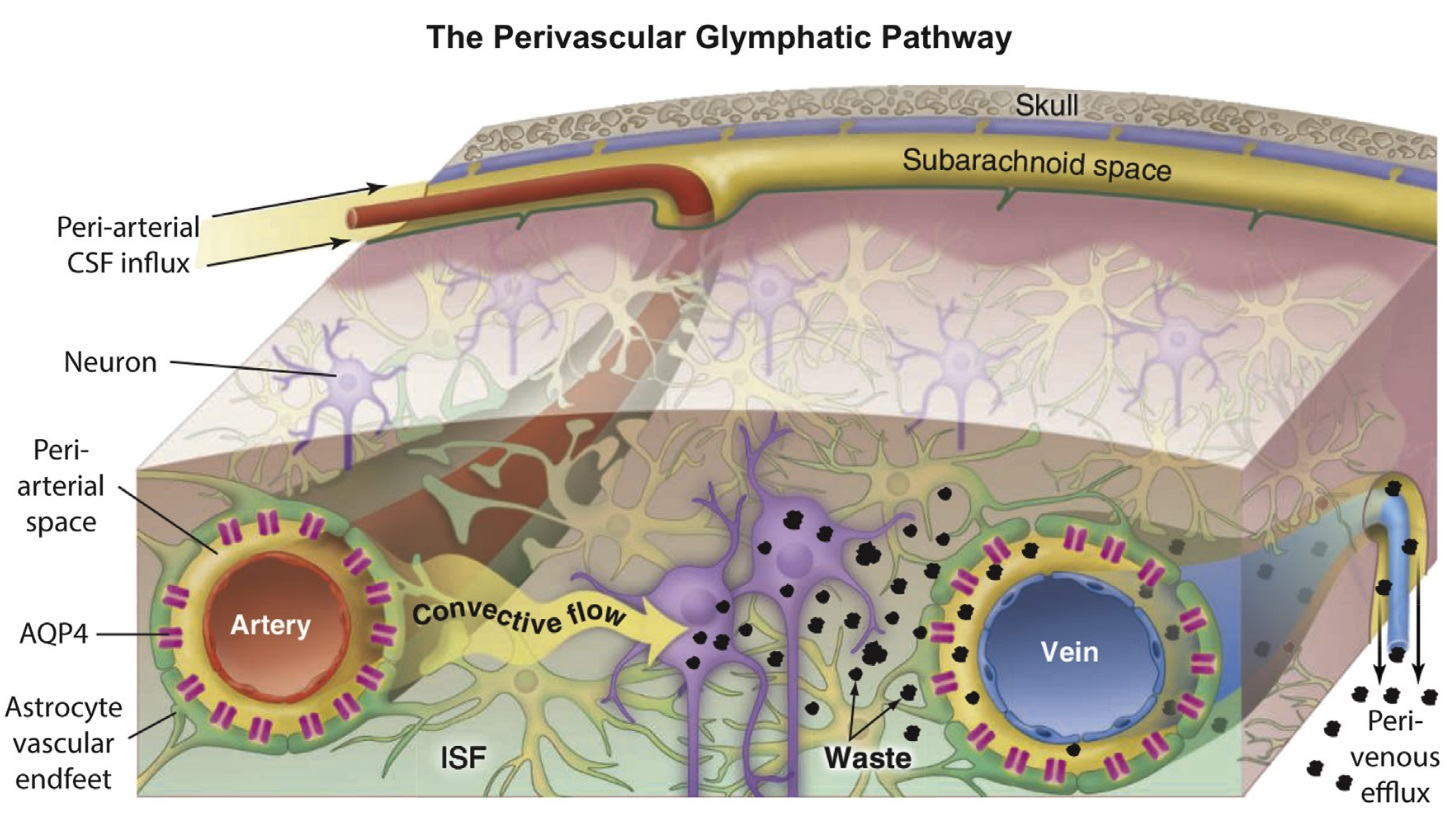
\includegraphics[scale = .6]{Figures/Iliff_2017_GlymphaticSystem.jpg}
    \caption{Diagram of the glymphatic system \citep{Nedergaard2013}}
  \label{fig:glym}
\end{figure}

One of the most important findings about the glymphatic system is its potential mechanistic link with AD. Along with other metabolites, glymphatic activity increases the clearance of both A$\beta$ and tau \citep{Iliff2012, Iliff2014, Xie}. Furthermore, this link is bidirectional, in the TgArcSwe mouse model of AD AQP4 polarization to endfeet was suppressed, and a similar effect has been shown to occur with age \citep{Yang2013, Kress2014, Zeppenfeld2017}. In another mouse model, AD APP/PS1, it was shown that glymphatic failures preceeds deposits of A$\beta$, but also that A$\beta$ exacerbates the issue by further inhibiting flow \citep{Peng2016}.

%Traumatic brain injury reduces glymphatic clearance by around 60$\%$. Impairing glymphatic system promotes tau pathology following TBI. AQP4 knockouts increase neurodegeneration and inflammation following TBI. Reactive astrocytes have reduced polarity of AQP4 disrupting perivascular structure. \citep{Iliff2014}

%%%%%%%%%%%%%%%%%%%%%%%%%%%%%%%%%%%%%%%%%%%%%%%%%%%%%%%%%%%%%%%%%%%%%%%%%%%%%%%%%%%%
%%%%%%%%%%%%%%%%%%%%%%%%%%%%%%%%%%%%%%%%%%%%%%%%%%%%%%%%%%%%%%%%%%%%%%%%%%%%%%%%%%%%
\section*{Aging and Alzheimer's Disease}
%%%%%%%%%%%%%%%%%%%%%%%%%%%%%%%%%%%%%%%%%%%%%%%%%%%%%%%%%%%%%%%%%%%%%%%%%%%%%%%%%%%%
%%%%%%%%%%%%%%%%%%%%%%%%%%%%%%%%%%%%%%%%%%%%%%%%%%%%%%%%%%%%%%%%%%%%%%%%%%%%%%%%%%%%
\subsection*{Amyloid-$\beta$ and Tau}
Since Alzheimer's dementia was first described by Alois Alzheimer as presenile and senile dementia, it has been diagnosed by the presence of senile plaques and neurofibrillary tangles, which were later discovered to be protein aggregates of amyloid-$\beta$ (A$\beta$) and phosphorylated tau \citep{Berrios1990}. Both A$\beta$ and tau are proteins associated with normal brain activity, but the accumulation of the protein aggregates are toxic.

A$\beta$ is formed when amyloid precursor protein (APP) is embedded in a cell's membrane and subsequently cleaved by $\beta$- and $\gamma$- secretases\citep{Vassar1999}. The protein is found in various cells of the body, and is particularly concentrated in the synapses of neurons \citep{Priller2006a}. Although the native role of APP has remained elusive, there are suggestions that it may be necessary for neuronal migration, the correct functioning of synapses, and cell adhesion \citep{Mattson1997,Young-Pearse2007,Priller2006a}. 

%**
Tau, the protein responsible for the formation of tangles is a microtubule associated protein, which stabilizes the formation microtubule \citep{Wang2016}. However, when it becomes phosphorylated, it is no longer able to stabilizes the microtubules. It can become misfolded making it insoluble, and form aggregate, or tangles \citep{Iqbal2016}. These tangles are especially pathogenic because they are able to spread to nearby neurons, and like a prion, cause more tangles to form.

%**
\subsection*{Sleep and aging}
Older adults encounter problems with sleep which worsen age; for instance, it takes longer to fall asleep, sleep decreases in duration, awakenings occur more frequently throughout the night and more readily in response to disturbances, and most of sleep is spent in NREM1 $\&$ 2 (rather than NREM3 or REM). Somewhat unsurprisingly, older populations report more daytime sleepiness and engage in unplanned naps. Both the power and quantity of SWs as well as spindles are reduced with age.\citep{Mander2017} Furthermore, the typical coupling of spindles with SWs that is correlated with memory consolidation is reduced in older adults \citep{Helfrich2018}. Time spent awake, increases homeostatic sleep pressure, and if sleep deprivation is sufficiently prolonged SW activity increases and is correlated with lapses in performance on cognitive tasks humans.\citep{Rodriguez2016,Watson2016,Nir2017}. Amyloid-$\beta$ accumulates with time spent awake \citep{Bateman2006,Kang2009, Xie Mander2015}%[and tau?]

%%%%%%%%%%%%%%%%%%%%%%%%%%%%%%%%%%%%%%%%%%%%%%%%%%%%%%%%%%%%%%%%%%%%%%%%%%%%%%%%%%%%
%%%%%%%%%%%%%%%%%%%%%%%%%%%%%%%%%%%%%%%%%%%%%%%%%%%%%%%%%%%%%%%%%%%%%%%%%%%%%%%%%%%%
%Trash
%%%%%%%%%%%%%%%%%%%%%%%%%%%%%%%%%%%%%%%%%%%%%%%%%%%%%%%%%%%%%%%%%%%%%%%%%%%%%%%%%%%%
%%%%%%%%%%%%%%%%%%%%%%%%%%%%%%%%%%%%%%%%%%%%%%%%%%%%%%%%%%%%%%%%%%%%%%%%%%%%%%%%%%%%
%Tonic activation of CMT causes NREM-wake transitions, while burst stimulation firing resembles up states in cingulate and promotes SW actiivty. Up-states are preceeded by firing in centromedial thalamus neurons. \citep{Gent2018}
%Ventromedial thalamic nucleus activity is low during NREM, increases during NREM-wake transition and stimulation induces a NREM-wake transition, caused activity in anesthesized animals, but did not disrupt REM sleep. \citep{Honjoh2018}

%% Staging
% These scoring criteria (with some slight modifications for other animals), have provided the standard framework to further study sleep. For instance, these are the stages used by clinicians to diagnose sleep disorders, and to study sleep induced biochemical changes. Likewise, this system has been a powerful influence on our understanding of sleep. While this standardization provides a common language for sleep necessary for building knowledge in this domain, it also creates a certain rigidity. The scoring criteria has remained essentially unchanged until 2007, when the AASM consolidated NREM3 and NREM4 into NREM3. While useful, a rigid framework may also impose artificial constraints scientific questions.
%%
%% Waves
%The body is composed of many cells of various types communicating with others at various distances and timescales. Most cells communicate by releasing signaling molecules. These signals can be passed almost immediately to a cell’s direct neighbors if there are gap junctions linking the cells; otherwise, the signal must diffuse through the extra-cellular space to reach its destination. A random walk through the tightly packed extracellular space means that the probability of a signal reaching a particular cell within some period of time falls off very quickly with distance. This problem is mitigated by the many vessels in the body providing less hindered directed channels of flow, and often propulsion to increase the speed. Although the neuron is subject to the same constraints, but it is exceptional in its ability to communicate quickly and at long distances because of a few remarkable adaptations. First, neurons leverage fast ionic conductivity by manipulating electrostatic and concentration gradients with dynamically tuned micro-fluidics. Second, some neurons have highly elongated processes which can grow to very long distances. These are far from the only remarkable features of neurons, but together, these adaptations effectively allow neurons to communicate with very distant cells as if they were next-door neighbors. While the evolutionary importance of features can hardly be overstated, the majority of neurons communicate over relatively short distances.
%The brain is a physical system basically composed of cells that can integrate many inputs, and over some threshold, project signals as input to other cells. However, inputs can vary widely in function, some on short timescales by raising or lowering the cells membrane potential, or others in some way re-tuning the cell - e.g. RNA transcription. Furthermore, these neurons can be arranged to create circuits, which are organized together perform complex computations.
%This ionic conduction also enables scientists to monitor the activity of neurons with electrophysiology. Population activity 
%These neurons can be quickly and precisely altered by various ion channel proteins in the membrane. short to long distances  physical system composed of many cells with different conductances that can integrate many inputs, and above some input threshold, project signals as input to other cells, and these cells 
%With extracellular electrophysiology, even for micro-electrodes capable of single unit recordings, it is difficult to determine the type of input or output.  of groups of neurons synchronizes to form oscillatory rhythms. 
%So, unless there is another source of the EEG signal besides neuronal activity, a global SW would entail that many widely distributed neurons are simultaneously activated and deactivated. Probably the easiest way to coordinate this would be for a single generator to send a signal to every area; however, conduction speed would lead to imprecise delivery times, unless this generator were located precisely the same distance from each region or somehow tuned to compensate for conduction.
%In contrast, a perfectly local signal would be one that is isolated to a single area, and not spread to other areas. In a less strict interpretation, a local signal might be one that occurs in one location, but could be sent to another location. This is unlikely because nearby areas are more highly connected.%Perhaps particular waveforms are emerge out of reaction diffusion stability. The detection of travelling waves could be used to infer effective connectivity. If this is the case, mapping the spatiotemporal repertoire of these waveforms may suggest its principal source and sinks, functional/computational role, facilitate a predictive model, etc. 
%So it is much more likely that there is a spread of activity into surrounding areas in addition to saltatory transmissions of activity to more remote areas, which in turn spread locally.
%The brain has very neurotransmitters, some with very exotic downstream effects, but on short-timescales most of them impart a transient change in ionic permeability increasing (excitatory) or decreases (inhibitory) voltage, and likewise firing probability. Furthermore, the connectivity of the neurons imparts a structure over which the excitatory and inhibitory signals can propagate. The dynamics of this system have been characterized as a reaction-diffusion system, which was famously introduced and analyzed by Alan Turing \citep{Turing1952}
%One of the most interesting features, of such systems are their extensive repertoire of spatiotemporal dynamics. Even simple systems can be tuned to reproduce patterns like leopard spots, and over time these patterns evolve as traveling waves of patterns

%% SW
% The up and down state can be partially explained by afterhyperpolarizations produced by Ca$^{2+}$ mediated increases in K$^+$ conductance in soma [47,48].
% Bereitschatfspotential, or readiness potentials, associated with surprise or initiation of movement cause synchronized afterhyperpolarizations which can produce a SW [50,51].
% Synchronized bursting pyramidal cells during NREM produce large dipole from positive infragranular and negative supragranular layers [48, 54-56].
% interneurons and thalamocortical inputs to pyramidal cells are active during down states [52,53,57,58]. 
% Cyclic nucleotide-gated hyperpolarization deinactivated (I$_h$) and low-voltage hyperpolarization-induced T-type Ca$^{2+}$ channels (I$_T$) create intrinsic cell resonance and produce oscillations of membrane potential which are unrelated to synaptic events [39]. In pyramidal cells this may produce theta rhythms [41-44], while in interneurons this may produce gamma rhythms [45,46]
% \citep{Buzsaki2012}
% Slow-waves are believed to emerge from the interactions between the cortex and the thalamus.
% Low-voltage gated T-type Ca$^{2+}$ channels cause low-threshold spike (LTS) Ca$^{2+}$ spikes causing rhythmic bursting with intraspike frequencies between 100-500Hz. 
% In contrast, alpha and theta waves are thought to be driven by both high-threshold spikes produced by both low T-type and high L-type voltage-gated Ca$^{2+}$ channels causing lower frequency bursting between 50-70 Hz.
% The source of EEG are supragranular cortical cells, but these involve thalamocortical interaction.
% While, \textit{in vivo} thalamic neurons produce only short delta oscillations, in decorticated animals, these oscillations are sustained (consistent with cortical disfacilitation during down states) [21-24].
% Unlike cortex, delta oscillations in the thalamic neuron rely on LTS bursts [4,20,25]
% "conclusively demonstrated in anesthetized and sleeping animals that SW EEG requires thalamic participation" [30, 37], but in isolation distinct mechanisms produce SW.
% SW are significantly reduced if synaptic transmission is blocked [21,22,38]
% TC neurons generated SW with K$^+$ leak, I$_T$, I$_{CAN}$, and I$_h$ [9, 11, 17, 39]. NRT neurons are similar, but also require Na$^2+$ and Ca$2+$ activated K$^+$ currents [34]. Furthermore, these can be transformed into delta rhythms with by changing the membrane potential via I$_T$ [11,17,39]. Notably, delta oscillations can occur during SW [5,6,9,34].
% \citep{Crunelli2018} 

%%Memory
%Nevertheless, it seems that during down states CA3 and CA1 are able to generate gamma bursts and ripples.
%Recurrent local circuits of deep cortical layers may produce SW and synchronize large swaths of cortex via long-range cortical connections in superficial layers. They hypothesize that an excitatory front of the SW spreads from cortex to entorhinal cortex to hippocampus, which is supported by consistent delay times. An important physiological role of SW is to coordinate locally emerging patterns. Integration and Segregation of Activity in Entorhinal-Hippocampal Subregions by Neocortical Slow Oscillations\cite{Isomura2006}
%Network homeostasis and State Dynamics of Neocortical Sleep \citep{Watson2016}
%IEDs hijack ripple band in rodent epilepsy models and associated with reduced memory consolidation. These IEDs induce SWs. \citep{Gelinas2016}

%CA
%Astrocyctes induce neuronal hyperpolarization via decreasing K$^+$ associated with Ca$2+$ signaling which increases signal to noise ratio of synaptic transmission. \citep{Wang2012}
% Reduced spontaneous as well as stimulation and agonist induced local somatic and process transients in addition to global, synchronized Ca$2+$ transients. Signaling in astrocytes is reduced temporally before neurons and at lower doses. While astrocytic Ca$2+$ signaling is critically dependent on IP3R2, it was only slightly reduced when neuronal signalling was blocked. \citep{Thrane2012}
%Astrocytic phagocytosis increases with sleep deprivation.

%% General
%The consequences of sleep deprivation are a growing list including loss of sex drive, elevated blood pressure, weakened immunity, cognitive impairment, and increased risk for a wide range of diseases. So while unconsciousness is the most obvious feature of sleep, it is just a side-effect of this profound state change which facilitates critical homeostatic processes throughout the body - especially in the brain. Around sleep onset, movement and sensory stimulation decrease, along with the demand for oxygen by the tissues serving these functions, thus permitting respiration to slow and the heart relax. As the brain falls deeper into sleep, the concentration of neuromodulatory transmitters, like norepinephrine and serotonin, decrease, and neuronal activity increasingly alternates between active and inactive firing states modulated by ~1 Hz waveforms called slow waves (SW). In parallel, astrocytes reduce their rate of anaerobic glycolysis, seek out synapses to phagocytose, and alter ionic composition of extracellular cerebrospinal fluid (CSF) in addition to permitting greater flow of CSF into/out of the brain. Importantly, these sleep processes and others have strong connections to cognition, aging, and disease, but some of these findings are inadequately studied in humans mostly limited by suitable methods that also meet the paramount ethical considerations for studying human subjects.
%Like the rest of nature, the life of an organism consists of persistent cycles interweaving with one another to support the whole.
%The development of the brain is a story of neurons and glia eventually emerging together as daughters of the gastrula's neural crest cells. These cells organize themselves into a complex pattern harmonizing with the parallel development of the vascular system and overcoming space constraints of the skull by folding as it continues to expand. Of course, this development does not stop after birth, but continues, albeit in a different way, as the organism adapts an environment and body in constant change.
%Importantly, during sleep as well as wake, neurons do not operate in isolation, but are supported by the entire body, and most intimately by its direct relatives the glia. Yet despite this critical dependence, studies of the human brain have a tendency to fixate on neural factors.
% Sleep is a great model to study interactions between brain systems because the activities of both neurons and glia change so markedly between these two states. Furthermore, sleep dysfunction is a risk factor for many diseases, especially of the brain. 
% I hope to identify mechanisms of interaction between systems supporting brain function by developing approaches that enhance existing imaging techniques through the integration of multiple data modalities.
% Longterm, homeostatic importance of sleep, and interaction of various systems to support the brain.
% I think the neuroscience of sleep is intimately related to the work of non-neuronal cells forming a robust infrastructure that supports the strenuous activity and intricate, but fragile structure of the nervous system.
%Later Antoine Louveau and Jonathan Kipnis showed evidence of a more traditional lymphatic vessel incorporated in the brain’s dura, which has been termed cerebral lymphatic vessels.

%Many synpatic sleep-need-index phosphoproteins (SNIPPS) which phosphorylate with wake and dephosphorylated during sleep. A phosphorylating protein called SIK3 drove sleep need by phosphylating SNIPPs. \citep{Wang2018}

%%% Local Variables: ***
%%% mode: latex ***
%%% TeX-master: "thesis.tex" ***
%%% End: ***

\mychapter{3}{Preliminary results}
%
% This section should include your research efforts. Appropriate discussion and methods are important; you should show how you can perform all of the necessary techniques and methods. Please embed figures into the text and include a brief legend. Figures and Tables must be absolutely clear and visible. 
%
%%%%%%%%%%%%%%%%%%%%%%%%%%%%%%%%%%%%%%%%%%%%%%%%%%%%%%%%%%%%%%%%%%%%%%%%%%%%%%%%%%%%
%%%%%%%%%%%%%%%%%%%%%%%%%%%%%%%%%%%%%%%%%%%%%%%%%%%%%%%%%%%%%%%%%%%%%%%%%%%%%%%%%%%%
\section*{Methods}
%%%%%%%%%%%%%%%%%%%%%%%%%%%%%%%%%%%%%%%%%%%%%%%%%%%%%%%%%%%%%%%%%%%%%%%%%%%%%%%%%%%%
%%%%%%%%%%%%%%%%%%%%%%%%%%%%%%%%%%%%%%%%%%%%%%%%%%%%%%%%%%%%%%%%%%%%%%%%%%%%%%%%%%%%

%%%%%%%%%%%%%%%%%%%%%%%%%%%%%%%%%%%%%%%%%%%%%%%%%%%%%%%%%%%%%%%%%%%%%%%%%%%%%%%%%%%%
\subsection*{Intracranial Encephalography (iEEG)}
%%%%%%%%%%%%%%%%%%%%%%%%%%%%%%%%%%%%%%%%%%%%%%%%%%%%%%%%%%%%%%%%%%%%%%%%%%%%%%%%%%%%
Hans Berger EEG
Nature of signal. Net activity of population – Locality, Number of cells, etc. Volume conduction. 
Medically intractable focal epilepsy. All patients are candidates for resective epilepsy surgery. Electrodes are implanted solely for the purpose of localizing.
Despite patients suffering from epilepsy, the majority physiological  
%[Cite: Origins of extracellular feilds - Buszaki, Anastassiou, & Koch, 2012]

%%%%%%%%%%%%%%%%%%%%%%%%%%%%%%%%%%%%%%%%%%%%%%%%%%%%%%%%%%%%%%%%%%%%%%%%%%%%%%%%%%%%
\subsection*{Network Connectivity}
%%%%%%%%%%%%%%%%%%%%%%%%%%%%%%%%%%%%%%%%%%%%%%%%%%%%%%%%%%%%%%%%%%%%%%%%%%%%%%%%%%%%
Functional connectivity involves characterizing the statistical relationship between brain signals, while anatomical connectivity is concerned with describing the way the physical components of the brain are physically connected. However, a mechanistic account of the brain involves describing how the anatomy causes its functional connectivity, and this so called effective connectivity consists of a model describing how the anatomical elements affect each other.

Probably the simplest way this could be accomplished is with a time dependent system of linear equations modeling the signals in each region as a function of the signals in the regions it is connected. In this sense, the method above is a measure of effective connectivity for local regions of the brain. Cortex is highly 

Contrast with other network connectivity measures, e.g. zero-lag correlation, phase-lag, etc. Lag threads.

“Therefore, the dynamical organization of rs-fMRI and its relation to brain states may manifest more fundamentally in spatiotemporal trajectories than changes in correlation structure.” (Mitra, 2018). “... our results suggest that—at least for the frequencies and regions we examined—the precise frequency of an oscillation could most closely relate to broad physiological factors such as the direction of wave propagation...The coexistence of traveling waves and CFC suggests that spatial bands of high-frequency neural activity move across the human cortex during behavior (Bahramisharif et al., 2013)” (Zhang, 2018)

%%%%%%%%%%%%%%%%%%%%%%%%%%%%%%%%%%%%%%%%%%%%%%%%%%%%%%%%%%%%%%%%%%%%%%%%%%%%%%%%%%%%
\subsection*{Traveling waves}
%%%%%%%%%%%%%%%%%%%%%%%%%%%%%%%%%%%%%%%%%%%%%%%%%%%%%%%%%%%%%%%%%%%%%%%%%%%%%%%%%%%%
\subsection*{Data preprocessing}
Re-referencing. Filtering. Artifact removal. SW and spindle detection.
Electrode localization. Surface mesh. 
\subsubsection*{Spatial embedding of electrodes}
Euclidean vs Geodesic distance. Electrode to mesh. Fast-marching algorithm. Transforming distance matrix to 3D coordinates.

\subsubsection*{Lag time network}
Peak lag. Lag of maximum correlation. 

%%% Local Variables: ***
%%% mode: latex ***
%%% TeX-master: "thesis.tex" ***
%%% End: ***

\mychapter{4}{Proposed work}
%
% The proposal should address the feasibility of various experiments and point out caveats that might be encountered and how these could be circumvented. Be sure to include positive and negative controls, analysis and interpretation, pitfalls and alternative approaches, and somewhat detailed methods. Prioritize
%
\section*{Name-face association task}
To investigate the effects of sleep on memory consolidation, I propose creating an audio-visual name-face association task administered such that training and testing phases are separated by an intervening period of sleep. 

%
% To that end, we have designed a task with rich audio-visual stimuli pairs, hippocampal dependent learning.
\subsection*{Stimuli}
The task involves learning associations between audio clips of a speaker introducing themselves and the picture of a face paired with that name. Names will be drawn from a database of names along with their frequencies in the US and California (https://www.ssa.gov/oact/babynames/). The audio of names will be spoken in a standard American English accent also with a neutral tone, and will be either recorded by voice actors or clipped from existing audio - for example on YouTube. Face stimuli will be high-quality color static images of people expressing a neutral affect, and featuring only the shoulders and above. The face will be set in front of a light backdrop and the images will be presented on a black background. Finally, any text will be presented with standard sans-serif font in white.  

\subsection*{Training}
During the training phase, subjects will be presented with 50 face-name pairs. Each presentation will be preceded by a white fixation cross on a black background for 100 ms. A face will then be presented, followed 500 ms later by an audio clip of the corresponding name. The face will remain on display for an additional 500 ms before it is followed by a screen prompting the subject to either (1) "repeat the name in your head" or (2) "imagine the face." The subject will be given 1000 ms before the next blank screen. 

\subsection*{Rehearsal}
%either the name or the face will be presented followed by a prompt 500 ms later. If the face is presented, the subject will be prompted to "say this person's name aloud" or (2) "say this persons name in your head." If the name was presented, the person will be prompted to "imagine this person's face." In either case, 1500 ms later, the correct name or face will follow. Rehearsal trials are designed to elicit memory reactivation, and by using varying prompts, we hope to identify how reactivation networks are recruited more generally.

\subsection*{Test}
A test phase will be administered immediately following training and again after sleep. During this phase, a face will be presented followed by a prompt to "say this person's name aloud" 500 ms later. No feedback will be given to indicate whether the subject was correct.

\subsection*{Sleep}
Before the final test session, subjects will be asked to sleep. Prior to them sleeping, a subset of five names will be selected to be played during sleep. A volume will be chosen that is slightly below that of casual speech so that the patient will not be woken.
% Random subjects or single unit response? Random played or cued by SW?
\cite{Sharon2017}

\subsection*{Subjects}
Although this task was designed for patients implanted with iEEG to probe fast network dynamics supporting to memory consolidation and reactivation during sleep, it need not be limited to this population. With few modifications it can be implemented for other populations to be studied using MRI and/or EEG. In fact, this task would be well suited to study AD patients, as memory for face-name associations is something that was previously shown to be predictive of amyloid burden.

\subsection*{Analyses}
Hypothesize task response will involve activity in near the superior lateral temporal lobe during name stimuli presentation. Then during face stimuli presentation, occipital lobe and fusiform gyrus activity will increase. We expect each of these activities to exhibit functional connectivity to the hippocampus and frontal lobe during imagined reactivation and.

\subsection*{Discussion}
Single units
Memory alzheimer's
Biographical memories
Interpersonal memories
Emotion - voice or expression.

\section*{Evaluating Glymphatic Activity in Humans}
With ongoing collaboration with the ADRC, I have access to a large cohort of patients with Alzheimer's Disease willing to participate in MRI scans. Preliminary analyses suggest that. A successful execution would enhance our basic model for how brain rhythms are coordinated in space and how this coordination supports memory. Additionally, we evidence of glymphatic clearance.

This method is specifically targeted to test the hypotheses that CSF flow into and out of brain parenchyma increases during slow wave sleep relative to wake. We expect the flow increase immediately surrounding arteries to have an increase oriented orthogonally from blood flow and into parenchyma, and vice-versa near the veins. We hypothesize these flows will occur rhythmically modulated by the cardiac cycle and respiratory cycle for the periarterial and perivenous voxels. Additionally, compared to healthy controls and patients with disease, we expect this CSF flow to be disrupted, both slower and less directed.



%%%%%%%%%%%%%%%%%%%%%%%%%%%%%%%%%%%%%%%%%%%%%%%%%%%%%%%%%%%%%%%%%%%%%%%%%%%%%%%%%%
%%%%%%%%%%%%%%%%%%%%%%%%%%%%%%%%%%%%%%%%%%%%%%%%%%%%%%%%%%%%%%%%%%%%%%%%%%%%%%%%%%
% TRASH
%%%%%%%%%%%%%%%%%%%%%%%%%%%%%%%%%%%%%%%%%%%%%%%%%%%%%%%%%%%%%%%%%%%%%%%%%%%%%%%%%%
%%%%%%%%%%%%%%%%%%%%%%%%%%%%%%%%%%%%%%%%%%%%%%%%%%%%%%%%%%%%%%%%%%%%%%%%%%%%%%%%%%
%\subsection*{Audiovisual learning}
% Ears. The conical shape of the ear helps to focus air pressure waves onto the eardrum. These vibrations in turn displace a system of three bone -- the malleus, incus, and stapes -- which has the effect of amplifying this signal concentrating this force onto the smaller area of the stapes which beats against the fluid filled chamber of the cochlea. The vibrations of the cochlear fluid propagate through its spiral shape which helps to separate the sound into its frequency components: low frequencies are able to travel the entire length of the spiral, whereas higher frequencies travel shorter distances. Hair cells are located along this chamber, and the vibration of these hairs is finally transduces the original mechanical signal into action potentials which are carried to the brain stem by the auditory nerve. [Brain stem pathway]
%
%Eventually, these signals reach the auditory cortex, where the sounds are believed to be perceived as tones of various frequencies. This sort of fourier sound representation then propagates to other areas to endow the stimulus with more complex perceptions; like the visual system, there are believed to be dorsal and ventral processing streams related to the perception of where and what the stimulus is, respectively.

%%% Local Variables: ***
%%% mode: latex ***
%%% TeX-master: "thesis.tex" ***
%%% End: ***

% ... and so on

% These commands fix an odd problem in which the bibliography line
% of the Table of Contents shows the wrong page number.
\clearpage
\phantomsection

% "References should be formatted in style most common in discipline",
% abbrv is only a suggestion.
\bibliographystyle{apalike}
%\bibliography{thesis}
\bibliography{mendeley_v2,extra}

% The Thesis Manual says not to include appendix figures and tables in
% the List of Figures and Tables, respectively, so these commands from
% the caption package turn it off from this point onwards. If needed,
% it can be re-enabled later (using list=yes argument).
\captionsetup[figure]{list=no}
\captionsetup[table]{list=no}

% If you have an appendix, it should come after the references.
%% The original template (from Trevor) had a custom \appendix command,
% but I found it to break figure/table counters. I'm not sure how
% reliable my fix is, so I ended up reverting back to the standard
% latex version, and renaming the custom command to \myappendix.  You
% can try both and see how things work out:
% 1) Call \appendix once, and then make each appendix a \chapter
% 2) Call \myappendix once, and then make each appendix a \section.

\appendix
\chapter{Appendix Title}

Supplementary material goes here. See for instance Figure
\ref{fig:quote}.

\section{Lorem Ipsum}

dolor sit amet, consectetur adipisicing elit, sed do eiusmod tempor
incididunt ut labore et dolore magna aliqua. Ut enim ad minim veniam,
quis nostrud exercitation ullamco laboris nisi ut aliquip ex ea
commodo consequat. Duis aute irure dolor in reprehenderit in voluptate
velit esse cillum dolore eu fugiat nulla pariatur. Excepteur sint
occaecat cupidatat non proident, sunt in culpa qui officia deserunt
mollit anim id est laborum.

\begin{figure}
  \centering
  \begin{tabular}{l}
    ``I am glad I was up so late,\\
    \quad{}for that's the reason I was up so early.''\\
    \em \footnotesize William Shakespeare (1564-1616), British
    dramatist, poet.\\
    \em \footnotesize Cloten, in Cymbeline, act 2, sc. 3, l. 33-4.
  \end{tabular}
  \caption{A deep quote.}
  \label{fig:quote}
\end{figure}


%%% Local Variables: ***
%%% mode: latex ***
%%% TeX-master: "thesis.tex" ***
%%% End: ***


\end{document}
